\documentclass{article}
\usepackage{geometry}
\usepackage{subcaption}
\usepackage{hyperref}
\usepackage[many]{tcolorbox}
\usepackage{graphicx}
\usepackage{natbib}
\usepackage{amsmath}
\usepackage{xcolor}
\usepackage[utf8]{inputenc}
\usepackage{listings}
\usepackage{tikz,pgf,xcolor}
\usetikzlibrary{arrows,automata,trees,plotmarks,shadows,shapes,positioning}
\usepackage{pgfplots}
\usetikzlibrary{pgfplots.groupplots}
\usetikzlibrary{petri}
\usepackage{nicefrac}
\setlength\parindent{0pt}
\usepackage{authblk}
\renewcommand\thesubsection{\alph{subsection})}
\geometry{a4paper,}

\definecolor{darkcandyapplered}{rgb}{0.64, 0.0, 0.0}
\definecolor{ao}{rgb}{0.0, 0.5, 0.0}
\definecolor{ghostwhite}{rgb}{0.93, 0.93, 0.93}
\definecolor{darkpowderblue}{rgb}{0.0, 0.2, 0.6}
\definecolor{deepcarrotorange}{rgb}{0.91, 0.41, 0.17}
\definecolor{rebeccapurple}{rgb}{0.28, 0.24, 0.54}

\hypersetup{
  colorlinks   = true, %Colours links instead of ugly boxes
  urlcolor     = darkpowderblue, %Colour for external hyperlinks
  linkcolor    = darkpowderblue, %Colour of internal links
  citecolor   = darkcandyapplered %Colour of citations
}

\lstdefinestyle{CL}
{
backgroundcolor=\color{ghostwhite},
basicstyle=\footnotesize\color{black}\ttfamily,
moredelim=**[is][\color{darkcandyapplered}]{@}{@},
moredelim=**[is][\color{ao}]{&}{&},
moredelim=**[is][\color{darkpowderblue}]{!}{!},  
moredelim=**[is][\color{deepcarrotorange}]{~}{~},      
xrightmargin=-27pt,
%showlines=true,
}

\lstdefinestyle{DOS}
{
backgroundcolor=\color{black},
basicstyle=\scriptsize\color{white}\ttfamily
xleftmargin=-25pt,
xrightmargin=-25pt,
aboveskip=-.2 \baselineskip, 
%showlines=true,
}
\title{\textbf{Entropia 1.5 \\ \large User's Guide}} 
\author[1]{Artem Polyvyanyy}
\author[1]{Hanan Alkhammash}
\author[2]{Claudio Di Ciccio}
\author[3]{Luciano García-Bañuelos}
\author[1]{Anna Kalenkova}
\author[4]{Sander J. J. Leemans}
\author[5]{Jan Mendling}
\author[1]{Alistair Moffat}
\author[6]{Matthias Weidlich}
\affil[1]{The University of Melbourne}
\affil[ ]{\textit {\{artem.polyvyanyy,halkhammash,anna.kalenkova,ammoffat\}@unimelb.edu.au}}
\affil[2]{Sapienza University of Rome}
\affil[ ]{\textit {diciccio@di.uniroma1.it}}
\affil[3]{Tecnológico de Monterrey}
\affil[ ]{\textit {luciano.garcia@tec.mx}}
\affil[4]{Queensland University of Technology}
\affil[ ]{\textit {s.leemans@qut.edu.au}}
\affil[5]{Vienna University of Economics and Business}
\affil[ ]{\textit {jan.mendling@wu.ac.at}}
\affil[6]{Humboldt-Universität zu Berlin}
\affil[ ]{\textit {matthias.weidlich@hu-berlin.de}}
\date{}

\begin{document}
\maketitle 
Entropia is an open-source command-line tool that implements a family of conformance checking measures. This guide is intended to explains through a series of simple steps how to use the Entropia tool to measure precision and recall between a model and an event log using classical non-deterministic and stochastic conformance checking approaches. This guide covers the following topics:

\begin{enumerate}
\itemsep0em 
\item Getting Started: find out how to get Entropia and prerequisites required to run the tool.  
\item Classical Non-deterministic Conformance Checking Measures: The Entropia commands for the are provided where each command-line instruction is illustrated with an example, making it easy to find the information you are looking for. The section covers the following measures: 
\begin{enumerate}
\itemsep0em 
\item[1.] Exact Matching Precision and Recall \cite{Polyvyanyy2020TOSEM}, 
\item[2.] Partial Matching Precision and Recall \cite{PolyvyanyyK2019}; and
\item[3.] Controlled Partial Matching Precision and Recall \cite{KalenkovaP2020},
\end{enumerate}
\item The Entropia commands for stochastic conformance checking measures. Here, you can find out a detailed description you need to apply different stochastic conformance checking approaches. The section includes the following measures: 
\begin{enumerate}
\item[1.] Stochastic Precision and Recall  \cite{Leemans2020}; and
\item[2.] Entropic Relevance \cite{abs-2007-09310}. 
\end{enumerate}
\end{enumerate}

\newpage
\section*{Getting Started with Entropia}
\label{sec:start}
This section will quickly get you started in using the Entropia tool.

\subsection{Checking for prerequisite}
Prior to running the Entropia commands, you will need to ensure that the \textbf{JDK} (Java Development Kit) is in place.
\subsection{Downloading and Running Entropia}

\begin{enumerate}
\itemsep0em 
\item Clone or download the JPBT library to your local machine: \url{https://github.com/jbpt/codebase}.
\item Navigate to the jbpt-pm folder in your terminal.
\item Issue the following command to verify that the Entropia tool is properly downloaded and display its version number as shown in the output screen:
\end{enumerate}
\begin{lstlisting}[style=CL]
>java -jar !jbpt-pm-entropia-1.5.jar! @-v@
\end{lstlisting}
\textbf{Output Screen:}
\begin{lstlisting}[style=DOS]
>java -jar jbpt-pm-entropia-1.5.jar -v
1.5
\end{lstlisting}
\smallbreak
Use the option (\textcolor{darkcandyapplered}{\footnotesize\ttfamily-h}) to display the help message that shows information of the core and specific options of the Entropia tool.
\begin{lstlisting}[style=CL]
>java -jar !jbpt-pm-entropia-1.5.jar! @-h@
\end{lstlisting}
\textbf{Output Screen:}%chnage
\lstinputlisting[style=DOS]{screens/screen_(-h).txt}

\section*{Models and Event Log}
The tutorial will use example files that are provided with the tool, which are the event log coded in XES format (log.xes), process model modelled as a Petri Net (model.pnml) and stochastic process model as an SDFA coded in JSON format (automaton.json). Table 1, Figure 1 and Figure 2 represent the three files, respectively. 


\begin{figure}[h!]
\hspace{3mm}
 \begin{minipage}{0.45\textwidth}
\begin{center}
\vspace{-3mm}
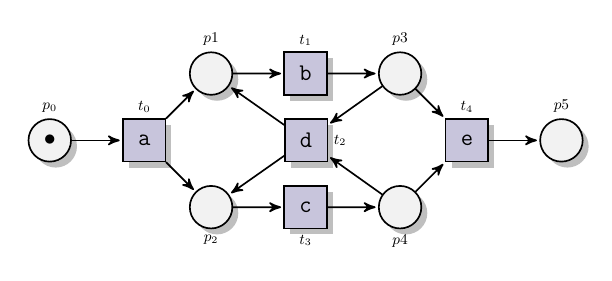
\begin{tikzpicture}[scale=0.6, transform shape, ->, >=stealth', shorten >=1pt, auto, node distance=20mm, on grid, semithick, transition/.style={fill=rebeccapurple!30, draw, minimum size=9mm, drop shadow}, place/.style={fill=black!5, draw, circle, minimum size=9mm, drop shadow}]

\node[place,label=90:\small $p_0$]				(p0) 											{\Large $\bullet$};
\node[transition,label=90:\small $t_0$]		(t0) [right=of p0] 				{\Large $\texttt{a}$};
\node[place,label=90:\small $p1$] 				(p1) [above right=of t0]	{};
\node[place,label=270:\small $p_2$] 			(p2) [below right=of t0]	{};
\node[transition,label=90:\small $t_1$] 	(t1) [right=of p1]				{\Large $\texttt{b}$};
\node[transition,label=270:\small $t_3$] 	(t3) [right=of p2]				{\Large $\texttt{c}$};
\node[transition,label=0:\small $t_2$] 		(t2) [below right=of p1,xshift=17pt]				{\Large $\texttt{d}$};
\node[place,label=90:\small $p3$] 				(p3) [right=of t1]				{};
\node[place,label=270:\small $p4$] 				(p4) [right=of t3]				{};
\node[transition,label=90:\small $t_4$] 	(t4) [below right=of p3]	{\Large $\texttt{e}$};
\node[place,label=90:\small $p5$] 				(p5) [right=of t4]				{};

\path (p0) edge node {} (t0)
			(t0) edge node {} (p1)
					 edge node {} (p2)
			(p1) edge node {} (t1)
			(p2) edge node {} (t3)
			(t1) edge node {} (p3)
			(t3) edge node {} (p4)
			(t2) edge node {} (p1)
					 edge node {} (p2)
			(p3) edge node {} (t2)
					 edge node {} (t4)
			(p4) edge node {} (t2)
					 edge node {} (t4)
			(t4) edge node {} (p5)
;
\end{tikzpicture}
\vspace{-2mm}
\caption{Process Model.}
\label{fig:petri:net}
\vspace{-2mm}
\end{center}
\end{minipage}
\hspace{7mm}
\begin{minipage}{0.45\textwidth}
\begin{center}
\vspace{-9mm}
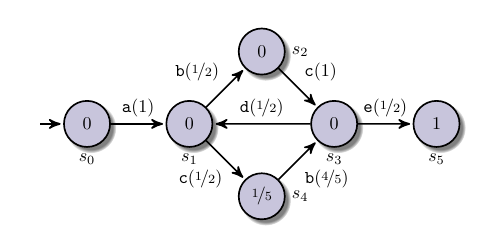
\begin{tikzpicture}[scale=0.65, transform shape, ->, >=stealth', shorten >=1pt, auto, initial text=, node distance=20mm, on grid, semithick, every state/.style={fill=rebeccapurple!30, draw, circular drop shadow, text=black, minimum size=9mm}]
\node[initial,state,label=270:$s_0$]	(s0) 											{$0$};
\node[state,label=270:$s_1$]					(s1) [right=of s0] 				{$0$};
\node[state,label=0:$s_2$]						(s2) [above right=of s1]	{$0$};
\node[state,label=270:$s_3$] 					(s3) [below right=of s2]	{$0$};
\node[state,label=0:$s_4$] 					  (s4) [below right=of s1]	{$\nicefrac{1}{5}$};
\node[state,label=270:$s_5$] 				  (s5) [right=of s3]				{$1$};

\path (s0) edge node {$\texttt{a}(1)$} (s1)
			(s1) edge node {$\texttt{b}(\nicefrac{1}{2})$} (s2)
			     edge node[below, xshift=-14pt, yshift=-2pt] {$\texttt{c}(\nicefrac{1}{2})$} (s4)
			(s2) edge node {$\texttt{c}(1)$} (s3)
			(s3) edge node[above]  {$\texttt{d}(\nicefrac{1}{2})$} (s1)
					 edge node {$\texttt{e}(\nicefrac{1}{2})$} (s5)
			(s4) edge node[below, xshift=16pt, yshift=-2pt] {$\texttt{b}(\nicefrac{4}{5})$} (s3);
\end{tikzpicture}
\vspace{3.5mm}
\caption{Stochastic Process Model.}
\label{fig:SDFA}
\vspace{-10mm}
\end{center}
\end{minipage}

\begin{center}
\vspace{5mm}
\begin{minipage}{0.45\textwidth}
 \centering
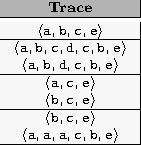
\includegraphics[width=0.40\textwidth]{fig/eventLog.pdf} 
\caption*{ Table 1: Event Log}
\label{fig:Log}
\end{minipage}
\end{center}
\vspace{-4mm}
\end{figure}

All files are located in the folder \textbf{jbpt-pm\slash guide\slash examples}. If the folder does not contain the files, you can download them from \url{https://github.com/jbpt/codebase/tree/master/jbpt-pm/entropia/guide/}. It is recommended to use the event log and models provided to understand how to run the Entropia commands. Then, try it with your own data. Refer to Table III in the demo paper for more details about file types and formats supported by the tool.

\section*{Classical Non-Deterministic Conformance Checking Measures}
\setcounter{subsection}{0}
\subsection{Matching Precision and Recall Measures}
To compute the exact matching precision value between the event log (log.xes) and process model  (model.pnml), use the option (\textcolor{darkcandyapplered}{\footnotesize\ttfamily-emp}) as follows.
\begin{lstlisting}[style=CL]
>java -jar !jbpt-pm-entropia-1.5.jar! @-emp@ &-rel=&log.xes &-ret&=model.pnml
\end{lstlisting}
Note that in the command the paths to the event log and process model files are assigned to the relevant (\textcolor{ao}{\footnotesize\ttfamily-rel=}\textcolor{gray}{\footnotesize\ttfamily<path>}) and retrieved (\textcolor{ao}{\footnotesize\ttfamily-ret=}\textcolor{gray}{\footnotesize\ttfamily<path>}) models respectively.\\

\textbf{Output Screen:}%chnage
\lstinputlisting[style=DOS]{screens/screen_(-emp).txt}

When the option (\textcolor{orange}{\footnotesize\ttfamily-s}) is added to commands, the tool runs in the silent mode. The following command is an example of using the (\textcolor{orange}{\footnotesize\ttfamily-s}) option:
\begin{lstlisting}[style=CL]
>java -jar !jbpt-pm-entropia-1.5.jar! @-emp@ ~-s~ &-rel=&log.xes &-ret=&model.pnml
\end{lstlisting}
The tool, in the silent mode, only prints the result, in this case the exact matching precision, omitting the debug information and execution data. The expected output of the command will be as the following. \\
%will be placed on the output screen
\textbf{Output Screen:}%chnage
\lstinputlisting[style=DOS]{screens/screen_(-emp-s).txt}

By replacing the option (\textcolor{darkcandyapplered}{\footnotesize\ttfamily-emr}) with (\textcolor{darkcandyapplered}{\footnotesize\ttfamily-emp}), the tool computes the exact matching recall value between the event log and process model. 

\begin{lstlisting}[style=CL]
>java -jar !jbpt-pm-entropia-1.5.jar! @-emr@ &-rel=&log.xes &-ret=&model.pnml
\end{lstlisting}
\textbf{Output Screen:}%chnage
\lstinputlisting[style=DOS]{screens/screen_(-emr).txt}

\subsection{Partial Matching Precision and Recall Measures}
To measure the partial matching precision value between the event log and model, use the option (\textcolor{darkcandyapplered}{\footnotesize\ttfamily-pmp}) on the command line followed by the paths to log (\textcolor{ao}{\footnotesize\ttfamily-rel=}\textcolor{gray}{\footnotesize\ttfamily<path>}) and model files (\textcolor{ao}{\footnotesize\ttfamily-ret=}\textcolor{gray}{\footnotesize\ttfamily<path>}), as follows: 
\begin{lstlisting}[style=CL]
>java -jar !jbpt-pm-entropia-1.5.jar! @-pmp@ ~-s~ &-rel=&log.xes &-ret=&model.pnml
\end{lstlisting}
\textbf{Output Screen:}(in the silent mode).
%chnage
\lstinputlisting[style=DOS]{screens/screen_(-pmp-s).txt}
When you replace the option (\textcolor{darkcandyapplered}{\footnotesize\ttfamily-pmp}) with (\textcolor{darkcandyapplered}{\footnotesize\ttfamily-pmr}), the tool measures the partial matching recall value.
\begin{lstlisting}[style=CL]
>java -jar !jbpt-pm-entropia-1.5.jar! @-pmr@ &-rel=&log.xes &-ret=&model.pnml
\end{lstlisting}
Note that the option (\textcolor{orange}{\footnotesize\ttfamily-s}) is removed as the debug information and execution data are placed on the output screen. \\
\textbf{Output Screen:}
\lstinputlisting[style=DOS]{screens/screen_(-pmr).txt}

\subsection{Controlled Partial Matching Precision and Recall Measures}
In order to measure controlled partial matching precision and recall values, the options (\textcolor{darkcandyapplered}{\footnotesize\ttfamily-cpmp}) and (\textcolor{darkcandyapplered}{\footnotesize\ttfamily-cpmr}) are used, respectively. Both options should be followed by the paths to log (\textcolor{ao}{\footnotesize\ttfamily-rel}\textcolor{gray}{\footnotesize\ttfamily<path>}) and model files (\textcolor{ao}{\footnotesize\ttfamily-ret}\textcolor{gray}{\footnotesize\ttfamily<path>}); and (\textcolor{ao}{\footnotesize\ttfamily-srel=}\textcolor{gray}{\footnotesize\ttfamily<num>}) and (\textcolor{ao}{\footnotesize\ttfamily-sret=}\textcolor{gray}{\footnotesize\ttfamily<num>}) options to specify the number of allowed skips in relevant and retrieved traces. 

The following command computes the controlled partial matching precision value between the event log and model, where (\textcolor{darkcandyapplered}{\footnotesize\ttfamily-cpmp}) is applied with a maximum of 3 allowed skipped actions in a trace described by each of the event log and model.
\begin{lstlisting}[style=CL]
>java -jar !jbpt-pm-entropia-1.5.jar! @-cpmp@ &-srel=&3 &-sret=&3 &-rel=&log.xes &-ret=&model.pnml
\end{lstlisting}
\textbf{Output Screen:}%chnage
\lstinputlisting[style=DOS]{screens/screen_(-cpmp).txt}

Similarly, in the following command, (\textcolor{darkcandyapplered}{\footnotesize\ttfamily-cpmr}) is used to measure the  controlled partial matching recall value, where the maximal number of allowed skipped actions in traces in the event log (\textcolor{ao}{\footnotesize\ttfamily-srel}) and model (\textcolor{ao}{\footnotesize\ttfamily-sret=<num>}) are 2 and 3, respectively.
\begin{lstlisting}[style=CL]
>java -jar !jbpt-pm-entropia-1.5.jar! @-cpmr@ &-srel=&2 -sret=&3 &-rel=&log.xes& &-ret=&model.pnml
\end{lstlisting}
\textbf{Output Screen:}%chnage. 
\lstinputlisting[style=DOS]{screens/screen_(-cpmr).txt}

\section*{Stochastic Conformance Checking Measures}
\setcounter{subsection}{0}
\subsection{Stochastic Precision and Recall Measures}
To compute the stochastic precision value between the event log and the process model, use the option (\textcolor{darkcandyapplered}{\footnotesize\ttfamily-sp}) as follows.
\begin{lstlisting}[style=CL]
>java -jar !jbpt-pm-entropia-1.5.jar! @-sp@ & -rel=log.xes& &-ret=automaton.json&
\end{lstlisting}
\textbf{Output Screen:}%chnage
\lstinputlisting[style=DOS]{screens/screen_(-sp).txt}

Use the option (\textcolor{darkcandyapplered}{\footnotesize\ttfamily-sr}) instead of (\textcolor{darkcandyapplered}{\footnotesize\ttfamily-sp}) in order to get the stochastic recall value between the event log and process model. 
\begin{lstlisting}[style=CL]
>java -jar !jbpt-pm-entropia-1.5.jar! @-sr@ & -rel=log.xes& &-ret=automaton.json&
\end{lstlisting}
\textbf{Output Screen:}%chnage
\lstinputlisting[style=DOS]{screens/screen_(-sr).txt}
\subsection{Entropic Relevance Measure}
You can measure relevance of a stochastic process model to an event log using the option (\textcolor{darkcandyapplered}{\footnotesize\ttfamily-r}), as the following command shows. Note that the retrieved model is specified to the stochastic process model, i.e. the stochastic deterministic finite automaton (SDFA), in JSON format.

\begin{lstlisting}[style=CL]
>java -jar !jbpt-pm-entropia-1.5.jar! @-r@ &-rel=&log.xes &-ret=&automaton.json
\end{lstlisting}
\textbf{Output Screen:}%chnage
\lstinputlisting[style=DOS]{screens/screen_(-r).txt}


\newpage
\bibliographystyle{plain}
\bibliography{bib}
\end{document}
